% =============================================
% 导言区
% =============================================
\documentclass{xjtureport}

% =============================================
% 正文区
% =============================================

\begin{document}
	
	% ===导入实验报告封面==============================
	\begin{titlepage}
		
\includepdf[pages=-]{figures/实验2封面.pdf}
	\end{titlepage}
	
	% ===正文==============================
	
	\chapterinline{实验二：码型变换实验}
	
	\section{实验目的}
	\begin{enumerate}
		\item 熟悉 RZ、BNRZ、BRZ、CMI、曼彻斯特、密勒、PST 等常见码型变换的原理及工作过程；
		\item 观察并比较不同数字基带信号码型的波形特性；
		\item 分析不同码型的频谱分布、直流分量及位同步性能。
	\end{enumerate}
	
	\section{实验器材}
	西电通信与信息工程实验平台（半实物仿真系统）。
	
	%\section{实验原理}
	
	\section{实验内容}
	
	\subsection*{(1) 单极性不归零码（NRZ）}
	\begin{enumerate}[label=\roman*.]
		\item 通过鼠标在编码码型中选择“NRZ码”，点击“基带设置”按钮，将基带数据设置为：16bit，64K，然后修改16bit编码开关的值。用示波器通道1观测编码前基带数据2P6，用通道2观测编码数据3P6；尝试修改不同的编码开关组合，观测编码前后数据。将基带数据设置为“15-PN”，“64K”，观测编码前数据2P6和编码数据3P6，并记录波形。根据观测的编码前数据和编码后数据时序关系，分析编码时延。
		
		\textbf{实验结果与分析：}
		
		图中 CH1（黄色）为基带信号，CH2（蓝色）为 NRZ 编码结果，二者的电平保持一一对应关系。
		
		\begin{figure}[H]
			\centering
			% --- 子图1：16bit 组合1 ---
			\begin{subfigure}{0.31\linewidth}
				\centering
				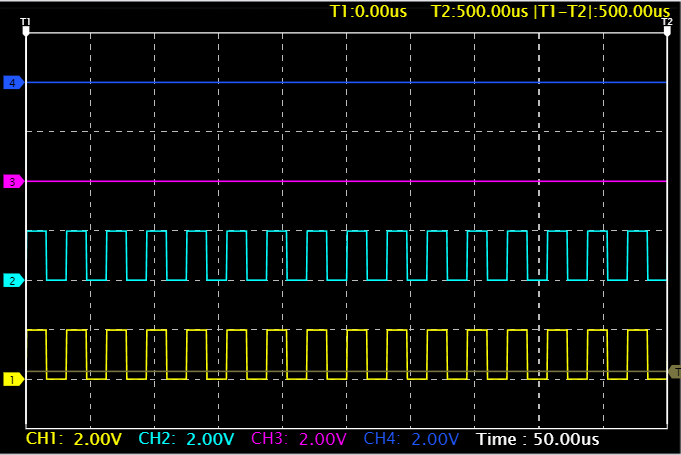
\includegraphics[width=\linewidth]{figures/16bit组合方式1输入下编码前后波形.png}
				\caption{16bit 组合方式一的编码前后波形（基带与编码）}
				\label{fig:nrz_16bit_case1}
			\end{subfigure}\hfill
			% --- 子图2：16bit 组合2 ---
			\begin{subfigure}{0.31\linewidth}
				\centering
				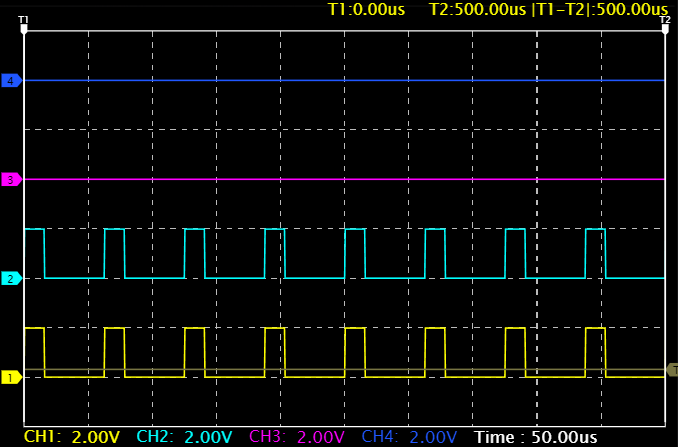
\includegraphics[width=\linewidth]{figures/16bit输入下编码前后波形.png}
				\caption{16bit 组合方式二的编码前后波形}
				\label{fig:nrz_16bit_case2}
			\end{subfigure}\hfill
			% --- 子图3：PN15 ---
			\begin{subfigure}{0.31\linewidth}
				\centering
				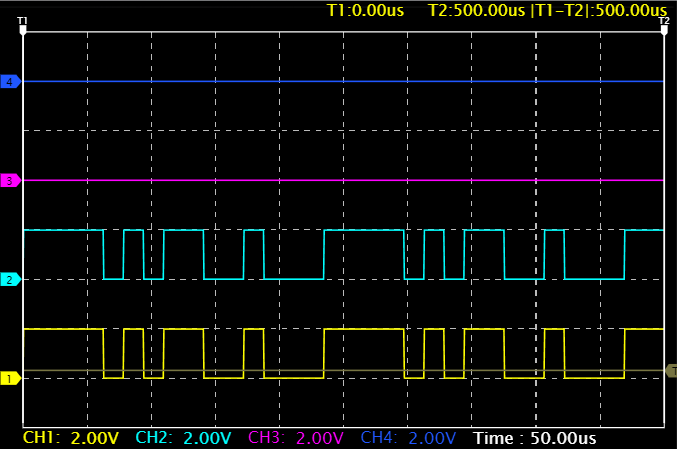
\includegraphics[width=\linewidth]{figures/PN15输入下的基带与 NRZ 编码波形.png}
				\caption{PN15 输入下的基带与 NRZ 编码波形}
				\label{fig:nrz_pn15}
			\end{subfigure}
			\caption{基带输入（CH1）与 NRZ 编码输出（CH2）的时域波形对比（时钟：64 kHz）}
			\label{fig:nrz_compare}
		\end{figure}
		
		\textbf{分析：}
		从图 \ref{fig:nrz_compare} 可以观察到：整体来看，NRZ 编码电路功能正常，编码后信号严格按规则映射，编码时延极小，可以忽略，认为无编码时延。
		
		\vspace{3em}
		
		\item 分析编码是否有直流分量？分析编码是否具备丰富的位同步信息（可设为全0码或全1码观测）。
		
		\textbf{实验结果：}
		
		\begin{figure}[H]
			\centering
			\begin{subfigure}{0.48\linewidth}
				\centering
				
\includegraphics[width=\linewidth]{全0码时的编码前后波形.png}
				\caption{全 0 码输入时的基带与 NRZ 编码波形}
				\label{fig:nrz_all0}
			\end{subfigure}\hfill
			\begin{subfigure}{0.48\linewidth}
				\centering
				
\includegraphics[width=\linewidth]{全1码时的编码前后波形.png}
				\caption{全 1 码输入时的基带与 NRZ 编码波形}
				\label{fig:nrz_all1}
			\end{subfigure}
			\caption{全 0 / 全 1 码输入下 NRZ 编码前后波形对比}
			\label{fig:nrz_dc_sync}
		\end{figure}
		
		\textbf{分析：}
		
		由图 \ref{fig:nrz_dc_sync} 可见，当输入为全 0 码时，编码输出始终为零电平；当输入为全 1 码时，编码输出始终为恒定高电平，说明 NRZ 码在一般情况下具有明显直流分量。由于在全 0 或全 1 情况下波形中几乎没有电平翻转，不包含可供提取的周期性成分，因此 NRZ 码不具备丰富的位同步信息。
		
		
		\vspace{3em}
		
		\item 分析编码前后，信号的频谱是否发生变化？
		
		\textbf{实验结果：}
		
		\begin{figure}[H]
			\centering
			\begin{subfigure}{0.48\linewidth}
				\centering
				
\includegraphics[width=\linewidth]{编码前波形频谱图.png}
				\caption{编码前基带信号的频谱}
				\label{fig:nrz_spec_before}
			\end{subfigure}\hfill
			\begin{subfigure}{0.48\linewidth}
				\centering
				
\includegraphics[width=\linewidth]{编码后波形频谱图.png}
				\caption{NRZ 编码后信号的频谱}
				\label{fig:nrz_spec_after}
			\end{subfigure}
			\caption{NRZ 编码前后信号频谱对比}
			\label{fig:nrz_spec_compare}
		\end{figure}
		
		\textbf{分析：}
		由图 \ref{fig:nrz_spec_compare} 可见，编码前后信号的频谱主瓣形状及能量分布基本一致。因此可认为编码前后频谱特性基本不变。
		
		
		\vspace{3em}
		
		\textbf{实验结果：}
		
		\begin{figure}[H]
			\centering
			% --- 组合1 ---
			\begin{subfigure}{0.48\linewidth}
				\centering
				
\includegraphics[width=\linewidth]{1_4基带组合1.png}
				\caption{16bit 组合方式一的基带输入（2P6）}
				\label{fig:nrz_decode_input1}
			\end{subfigure}\hfill
			\begin{subfigure}{0.48\linewidth}
				\centering
				
\includegraphics[width=\linewidth]{1_4基带组合1译码前后波形.png}
				\caption{组合方式一的译码输出（6TP3）与原基带对比}
				\label{fig:nrz_decode_output1}
			\end{subfigure}
			
			% --- 组合2 ---
			\begin{subfigure}{0.48\linewidth}
				\centering
				
\includegraphics[width=\linewidth]{1_4基带组合2.png}
				\caption{16bit 组合方式二的基带输入（2P6）}
				\label{fig:nrz_decode_input2}
			\end{subfigure}\hfill
			\begin{subfigure}{0.48\linewidth}
				\centering
				
\includegraphics[width=\linewidth]{1_4基带组合2译码前后波形.png}
				\caption{组合方式二的译码输出（6TP3）与原基带对比}
				\label{fig:nrz_decode_output2}
			\end{subfigure}
			
			\caption{NRZ 码在不同 16bit 组合下的编码前（2P6）与译码后（6TP3）波形对比}
			\label{fig:nrz_decode_compare}
		\end{figure}
		
		\textbf{分析：}
		由图 \ref{fig:nrz_decode_compare} 可见，译码后输出波形（6TP3）与编码前基带信号（2P6）在两种 16bit 组合下均完全一致，说明译码单元能够准确恢复原始基带数据。多次修改编码开关后，译码结果始终正确，表明系统的编码—译码链路工作稳定。
		
		从时序上看，译码输出相对于基带输入仅存在一个极小的固定延迟，该延迟由译码逻辑和同步时钟恢复电路引入，量级远小于一个码元周期，可认为译码时延可忽略。
		
		
		\vspace{3em}
	\end{enumerate}

	
	\subsection*{(2) 双极性不归零码（BNRZ）}
	本实验步骤与(1)单极性不归零码实验相同，所不同的是编码码型选择为“BNRZ码”。通过对比分析其波形特性及系统性能。
	
	\begin{enumerate}[label=\roman*.]
		\item 通过鼠标在编码码型中选择“BNRZ码”，点击“基带设置”按钮，将基带数据设置为：16bit，64K。修改16bit编码开关的值，用示波器通道1观测编码前基带数据2P6，用通道2观测编码数据3P6；尝试不同编码组合，记录波形。将基带数据设置为“15-PN”，“64K”，观测编码前数据2P6和编码数据3P6，并记录波形。根据观测的编码前数据和编码后数据时序关系，分析编码时延。
		
		\textbf{实验结果：}
		
		\begin{figure}[H]
			\centering
			\begin{subfigure}{0.31\linewidth}
				\centering
				
\includegraphics[width=\linewidth]{2_1 16bit组合方式1输入下编码前后波形.png}
				\caption{16bit 组合方式一时的基带与 BNRZ 编码波形}
				\label{fig:bnrz_16bit_case1}
			\end{subfigure}\hfill
			\begin{subfigure}{0.31\linewidth}
				\centering
				
\includegraphics[width=\linewidth]{2_1 16bit组合方式2输入下编码前后波形.png}
				\caption{16bit 组合方式二时的基带与 BNRZ 编码波形}
				\label{fig:bnrz_16bit_case2}
			\end{subfigure}\hfill
			\begin{subfigure}{0.31\linewidth}
				\centering
				
\includegraphics[width=\linewidth]{2_1 PN15输入下的编码前后波形.png}
				\caption{PN15 输入下的基带与 BNRZ 编码波形}
				\label{fig:bnrz_pn15}
			\end{subfigure}
			\caption{BNRZ 码下基带输入（2P6）与编码输出（3P6）的时域波形对比}
			\label{fig:bnrz_compare}
		\end{figure}
		
		\textbf{分析：}
		从图 \ref{fig:bnrz_compare} 可以观察到：BNRZ 编码将比特“1”和“0”分别映射为幅度相等、极性相反的正负电平，输出波形严格符合双极性不归零码的编码规则；在不同 16bit 组合和 PN15 输入下，编码后的波形仅随比特序列变化，其上升沿与基带数据基本对齐，说明编码电路工作正常，编码时延极小，可近似认为无译码时延。
		
		
		\vspace{3em}
		
		\item 分析编码是否有直流分量？分析编码是否具备丰富的位同步信息（可设为全0码或全1码观测）。
		
		\textbf{实验结果：}
		
		\begin{figure}[H]
			\centering
			\begin{subfigure}{0.48\linewidth}
				\centering
				
\includegraphics[width=\linewidth]{2_2 全0码时的编码前后波形.png}
				\caption{全 0 码输入时的基带与 BNRZ 编码波形}
				\label{fig:bnrz_all0}
			\end{subfigure}\hfill
			\begin{subfigure}{0.48\linewidth}
				\centering
				
\includegraphics[width=\linewidth]{2_2 全1码时的编码前后波形.png}
				\caption{全 1 码输入时的基带与 BNRZ 编码波形}
				\label{fig:bnrz_all1}
			\end{subfigure}
			\caption{全 0 / 全 1 码输入下 BNRZ 编码前后波形对比}
			\label{fig:bnrz_dc_sync}
		\end{figure}
		
		\textbf{分析：}
		双极性不归零码中，比特“1”和“0”分别映射为幅度相等、极性相反的正负电平。在随机数据、且“1”“0”等概出现的条件下，正负脉冲在时间上大致对称，平均值接近零，整体\textbf{可以认为基本不含直流分量}。但如图 \ref{fig:bnrz_dc_sync} 所示，当输入为全 0 或全 1 时，输出将长期保持恒定负电平或恒定正电平，此时会产生明显直流分量。
		
		由于 BNRZ 码码元之间同样不存在强制归零或固定翻转，当出现长时间连续“1”或“0”时，波形中缺乏电平跃迁，全 0 / 全 1 情况下几乎看不到边沿变化，因此\textbf{其位同步信息仍不丰富}。
		
		
		\vspace{3em}
		
		\item 分析编码前后，信号的频谱是否发生变化？
		
		\textbf{实验结果：}
		
		\begin{figure}[H]
			\centering
			\begin{subfigure}{0.48\linewidth}
				\centering
				
\includegraphics[width=\linewidth]{2_3 编码前波形频谱图.png}
				\caption{编码前基带信号的频谱}
				\label{fig:bnrz_spec_before}
			\end{subfigure}\hfill
			\begin{subfigure}{0.48\linewidth}
				\centering
				
\includegraphics[width=\linewidth]{2_3 编码后波形频谱图.png}
				\caption{BNRZ 编码后信号的频谱}
				\label{fig:bnrz_spec_after}
			\end{subfigure}
			\caption{BNRZ 编码前后信号频谱对比}
			\label{fig:bnrz_spec_compare}
		\end{figure}
		
		\textbf{分析：}
		
		从图 \ref{fig:bnrz_spec_compare} 可见，BNRZ 编码前后的频谱形状、主瓣宽度及整体分布基本一致，说明双极性不归零码同样属于基带幅度映射类编码，不会引入额外的频谱扩展或压缩。由于 BNRZ 输出不含明显直流成分，其在低频区域的能量略低于 NRZ，但与编码前基带信号相比变化很小，因此可认为 BNRZ 编码前后频谱特性基本保持不变。
		
		
		\vspace{3em}
		
		\item 使用双踪示波器，同时观测编码前数据2P6和译码后数据6TP3，观测编码前数据和译码后数据是否相同。尝试多次修改编码数据，观测译码数据是否正确。根据观测的编码前数据和译码后数据的时序关系，分析译码时延。
		
		\textbf{实验结果：}
		
		\begin{figure}[H]
			\centering
			\begin{subfigure}{0.48\linewidth}
				\centering
				
\includegraphics[width=\linewidth]{2_4基带组合1译码前后波形.png}
				\caption{16bit 组合方式一时的译码前后波形（2P6 与 6TP3）}
				\label{fig:bnrz_dec_case1}
			\end{subfigure}\hfill
			\begin{subfigure}{0.48\linewidth}
				\centering
				
\includegraphics[width=\linewidth]{2_4基带组合2译码前后波形.png}
				\caption{16bit 组合方式二时的编码前后波形}
				\label{fig:bnrz_dec_case2}
			\end{subfigure}
			\caption{BNRZ 码在不同 16bit 组合下的译码前数据与译码后数据对比}
			\label{fig:bnrz_dec_compare}
		\end{figure}
		
		\textbf{分析：}
		由图 \ref{fig:bnrz_dec_compare} 可见，在两种 16bit 组合下，译码后输出波形（6TP3）与编码前基带数据（2P6）一一对应，码型和比特序列完全一致，多次改变编码开关后译码结果仍保持正确，说明 BNRZ 编码/译码功能正常。两路信号上升沿之间仅存在固定的微小时间偏移，相比码元周期可以忽略不计，因此可认为译码时延很小，几乎无译码时延。
		
		
		
		\vspace{3em}
	\end{enumerate}
	
	
	\subsection*{(3) 单极性归零码（RZ）}
	本实验步骤与(1)相同，仅编码码型改为“RZ码”。通过对比NRZ码与RZ码的波形、直流分量和同步性能差异，总结归零操作对系统性能的影响。
	
	\begin{enumerate}[label=\roman*.]
		\item 设置编码码型为“RZ码”，基带数据为16bit、64K，修改16bit开关并记录波形。将基带数据改为“15-PN”，观测编码前2P6与编码后3P6信号，分析编码时延。
		
		\textbf{实验结果：}
		
		\begin{figure}[H]
			\centering
			\begin{subfigure}{0.31\linewidth}
				\centering
				
\includegraphics[width=\linewidth]{3_1 16bit组合方式1输入下编码前后波形.png}
				\caption{16bit 组合方式一时的基带与 RZ 编码波形}
				\label{fig:rz_16bit_case1}
			\end{subfigure}\hfill
			\begin{subfigure}{0.31\linewidth}
				\centering
				
\includegraphics[width=\linewidth]{3_1 16bit组合方式2输入下编码前后波形.png}
				\caption{16bit 组合方式二时的基带与 RZ 编码波形}
				\label{fig:rz_16bit_case2}
			\end{subfigure}\hfill
			\begin{subfigure}{0.31\linewidth}
				\centering
				
\includegraphics[width=\linewidth]{3_1 PN15输入下的编码前后波形.png}
				\caption{PN15 输入下的基带与 RZ 编码波形}
				\label{fig:rz_pn15}
			\end{subfigure}
			\caption{RZ 码下基带输入（2P6）与编码输出（3P6）的时域波形对比}
			\label{fig:rz_compare}
		\end{figure}
		
		\textbf{分析：}
		
		从图 \ref{fig:rz_compare} 可以看到，RZ 编码将比特“1”映射为在码元前半周期内的正电平脉冲，后半周期返回零电平，“0”始终为零电平。不同 16bit 组合及 PN15 输入下，编码后波形仅随比特序列变化，其上升沿与基带数据基本对齐，说明编码电路工作正常，编码时延极小，可近似认为无编码时延。
		
				
		\vspace{3em}
		
		\item 分析编码是否具有直流分量？是否具备丰富的位同步信息（可设为全0码或全1码进行验证）。
		
		\textbf{实验结果：}
		
		\begin{figure}[H]
			\centering
			\begin{subfigure}{0.48\linewidth}
				\centering
				
\includegraphics[width=\linewidth]{3_2 全0码时的编码前后波形.png}
				\caption{全 0 码输入时的基带与 RZ 编码波形}
				\label{fig:rz_all0}
			\end{subfigure}\hfill
			\begin{subfigure}{0.48\linewidth}
				\centering
				
\includegraphics[width=\linewidth]{3_2 全1码时的编码前后波形.png}
				\caption{全 1 码输入时的基带与 RZ 编码波形}
				\label{fig:rz_all1}
			\end{subfigure}
			\caption{全 0 / 全 1 码输入下 RZ 编码前后波形对比}
			\label{fig:rz_dc_sync}
		\end{figure}
		
		\textbf{分析：}
		RZ 码中，“1”码仅在码元前半周期输出正脉冲，后半周期归零；“0”码始终保持零电平。由于每个码元周期内电平都会回到零电平，\textbf{因此平均值较低，直流分量比 NRZ 小，但仍含直流分量}。
		
		从实验图 \ref{fig:rz_dc_sync} 可见：全 0 情况下输出始终为零电平；全 1 情况下输出为周期性短脉冲（脉宽为码元宽度的一半），而不会保持恒定高电平。  
		
		这一特性使得波形中持续存在固定频率的跃迁，\textbf{因此 RZ 码相比NRZ具有较丰富的位同步信息}。但是在全零码下仍缺少位同步信息。
		
		
		\vspace{3em}
		
		\item 分析编码前后信号频谱的变化情况。
		
		\textbf{实验结果：}
		
		\begin{figure}[H]
			\centering
			\begin{subfigure}{0.48\linewidth}
				\centering
				
\includegraphics[width=\linewidth]{3_3 编码前波形频谱图.png}
				\caption{编码前基带信号的频谱}
				\label{fig:rz_spec_before}
			\end{subfigure}\hfill
			\begin{subfigure}{0.48\linewidth}
				\centering
				
\includegraphics[width=\linewidth]{3_3 编码后波形频谱图.png}
				\caption{RZ 编码后信号的频谱}
				\label{fig:rz_spec_after}
			\end{subfigure}
			\caption{RZ 编码前后信号频谱对比}
			\label{fig:rz_spec_compare}
		\end{figure}
		
		\textbf{分析：}
		从图 \ref{fig:rz_spec_compare} 可见，与编码前相比，RZ 编码后的频谱在整体形状上仍保持基带信号的主瓣结构，但由于 RZ 码将“1”码压缩为半码元宽度的窄脉冲，使得信号的等效带宽增大，因此\textbf{高频成分相对增强，频谱扩展程度略高于编码前}。
		
		此外，RZ 码每个码元周期内都包含一次归零行为，因此直流成分显著下降，低频区域的能量明显低于编码前波形。总体来看，RZ 编码使频谱从低频区域部分迁移至较高频率，从而呈现出“低频成分减少、高频成分增强”的变化趋势。
		
		\vspace{3em}
		
		\item 使用双踪示波器观测编码前数据2P6与译码后数据6TP3，判断译码数据与原数据是否一致，并分析译码时延。
		
		\textbf{实验结果：}
		
		\begin{figure}[H]
			\centering
			\begin{subfigure}{0.48\linewidth}
				\centering
				
\includegraphics[width=\linewidth]{3_4基带组合1译码前后波形.png}
				\caption{16bit 组合方式一的译码前与译码后波形}
				\label{fig:rz_dec_case1}
			\end{subfigure}\hfill
			\begin{subfigure}{0.48\linewidth}
				\centering
				
\includegraphics[width=\linewidth]{3_4基带组合2译码前后波形.png}
				\caption{16bit 组合方式二的译码前后波形}
				\label{fig:rz_dec_case2}
			\end{subfigure}
			\caption{RZ 码在不同组合下的编码前数据与译码后数据对比}
			\label{fig:rz_dec_compare}
		\end{figure}
		
		\textbf{分析：}
		
		由图 \ref{fig:rz_dec_compare} 可见，译码输出（6TP3）在不同的 16bit 数据组合下均能准确恢复为原始基带数据（2P6），说明 RZ 码的译码电路工作正常，输出比特序列与输入完全一致。
		
		两路信号的上升沿位置仅存在极小的固有延迟，该延迟由译码单元的脉冲检测和同步时钟恢复造成。因此，RZ 译码的时延很小，可以认为几乎无译码时延。
		
		
		\vspace{3em}
	\end{enumerate}
	
	
	\subsection*{(4) 曼彻斯特码（Manchester）}
	本实验步骤与(1)相同，仅编码码型改为“曼彻斯特码”。通过实验对比观察其波形特征、同步性能和频谱分布。
	
	\begin{enumerate}[label=\roman*.]
		\item 通过鼠标在编码码型中选择“曼彻斯特码”，点击“基带设置”按钮，将基带数据设置为16bit，64K。修改16bit编码开关的值，用示波器通道1观测编码前基带数据2P6，用通道2观测编码数据3P6；尝试不同的编码组合，记录波形。将基带数据设置为“15-PN”，“64K”，观测编码前数据2P6和编码数据3P6，并记录波形。根据观测的编码前数据和编码后数据时序关系，分析编码时延。
		
		\textbf{实验结果：}
		
		\begin{figure}[H]
			\centering
			\begin{subfigure}{0.31\linewidth}
				\centering
				
\includegraphics[width=\linewidth]{4_1 16bit组合方式1输入下编码前后波形.png}
				\caption{16bit 组合方式一时的基带与曼彻斯特编码波形}
				\label{fig:man_16bit_case1}
			\end{subfigure}\hfill
			\begin{subfigure}{0.31\linewidth}
				\centering
				
\includegraphics[width=\linewidth]{4_1 16bit组合方式2输入下编码前后波形.png}
				\caption{16bit 组合方式二时的编码前后波形}
				\label{fig:man_16bit_case2}
			\end{subfigure}\hfill
			\begin{subfigure}{0.31\linewidth}
				\centering
				
\includegraphics[width=\linewidth]{4_1 PN15输入下的编码前后波形.png}
				\caption{PN15 输入下的基带与曼彻斯特编码波形}
				\label{fig:man_pn15}
			\end{subfigure}
			\caption{曼彻斯特码下基带输入（2P6）与编码输出（3P6）的时域波形对比}
			\label{fig:man_compare}
		\end{figure}
		
		\textbf{分析：}
		由图 \ref{fig:man_compare} 可见，曼彻斯特编码在每个码元内部都包含一次中间跳变：其中一半码元为正电平、另一半为负电平，且“0”“1”通过正负顺序的不同加以区分，符合数字双相码的编码规则。不同 16bit 组合及 PN15 输入下，编码输出在各比特边界与基带数据严格对应，仅存在极小的固定延时，因此可认为几乎无编码时延。
		
		\vspace{3em}
		
		\item 分析编码是否具有直流分量？分析编码是否具备丰富的位同步信息（可设为全0码或全1码观测）。
		
		\textbf{实验结果：}
		
		\begin{figure}[H]
			\centering
			\begin{subfigure}{0.48\linewidth}
				\centering
				
\includegraphics[width=\linewidth]{4_2 全0码时的编码前后波形.png}
				\caption{全 0 码输入时的基带与曼彻斯特编码波形}
				\label{fig:man_all0}
			\end{subfigure}\hfill
			\begin{subfigure}{0.48\linewidth}
				\centering
				
\includegraphics[width=\linewidth]{4_2 全1码时的编码前后波形.png}
				\caption{全 1 码输入时的基带与曼彻斯特编码波形}
				\label{fig:man_all1}
			\end{subfigure}
			\caption{全 0 / 全 1 码输入下曼彻斯特编码前后波形对比}
			\label{fig:man_dc_sync}
		\end{figure}
		
		\textbf{分析：}
		曼彻斯特码在每个码元中都包含一次硬性的中间跳变，且“1”“0”在码元前后半周期的极性相反，因此一个完整码元的平均值恒为零。由图 \ref{fig:man_dc_sync} 可见，无论输入为全 0 还是全 1，输出波形都呈现等宽的正负脉冲对称结构，\textbf{直流分量完全抵消，可认为不含直流成分}。
		
		此外，由于每个码元中都必定出现一次电平翻转，即使输入连续多个“0”或“1”，波形也始终包含固定频率的跳变，因此\textbf{曼彻斯特码具有极其丰富的位同步信息}。在实际系统中，它是一种典型的自同步码型，可以从信号本身稳定恢复时钟。
		
		
		\vspace{3em}
		
		\item 分析编码前后信号的频谱是否发生变化。
		
		\textbf{实验结果：}
		
		\begin{figure}[H]
			\centering
			\begin{subfigure}{0.48\linewidth}
				\centering
				
\includegraphics[width=\linewidth]{4_3 编码前波形频谱图.png}
				\caption{编码前基带信号的频谱}
				\label{fig:man_spec_before}
			\end{subfigure}\hfill
			\begin{subfigure}{0.48\linewidth}
				\centering
				
\includegraphics[width=\linewidth]{4_3 编码后波形频谱图.png}
				\caption{曼彻斯特编码后信号的频谱}
				\label{fig:man_spec_after}
			\end{subfigure}
			\caption{曼彻斯特编码前后信号频谱对比}
			\label{fig:man_spec_compare}
		\end{figure}
		
		\textbf{分析：}
		由图 \ref{fig:man_spec_compare} 可以看出，曼彻斯特编码后频谱整体形状仍呈带限基带特性，但由于每个码元内部必然出现一次翻转，相当于在原基带上叠加了一个与码元速率相关的方波成分，使得\textbf{高频成分相对增强，带宽略有扩展}。与编码前相比，有利于从频域中提取定时信息。
		
		
		\vspace{3em}
		
		\item 使用双踪示波器，同时观测编码前数据2P6与译码后数据6TP3，判断译码数据与原数据是否一致，并分析译码时延。
		
		\textbf{实验结果：}
		
		\begin{figure}[H]
			\centering
			\begin{subfigure}{0.48\linewidth}
				\centering
				
\includegraphics[width=\linewidth]{4_4基带组合1译码前后波形.png}
				\caption{16bit 组合方式一的译码前与译码后波形}
				\label{fig:man_dec_case1}
			\end{subfigure}\hfill
			\begin{subfigure}{0.48\linewidth}
				\centering
				
\includegraphics[width=\linewidth]{4_4基带组合2译码前后波形.png}
				\caption{16bit 组合方式二的译码前后波形}
				\label{fig:man_dec_case2}
			\end{subfigure}
			\caption{曼彻斯特码下不同组合的编码前与译码后波形对比}
			\label{fig:man_dec_compare}
		\end{figure}
		
		\textbf{分析：}
		由图 \ref{fig:man_dec_compare} 可见，不同 16bit 组合下，译码后输出波形（6TP3）与编码前基带数据（2P6）在比特序列上完全一致，说明曼彻斯特译码电路能够正确恢复原始数据。
		
		需要注意的是，译码后的波形整体相对于输入基带序列存在明显的\textbf{一个码元周期左右的固定延时}。这是由曼彻斯特码的结构决定的：每个码元的比特值需通过码元中点的强制跳变来判决，因此译码器必须等待码元周期的前半段结束后才能确定该码元的逻辑值，导致译码输出必然滞后约 1 bit。
		
		综上，曼彻斯特码译码结果正确，但译码存在\textbf{约一个码元周期的固有时延}，属于该码型的正常特性。
		
		
		\vspace{3em}
	\end{enumerate}
	
	
	\subsection*{(5) 密勒码（Miller）}
	本实验步骤与(1)相同，仅编码码型改为“密勒码”。重点分析密勒码在降低低频成分和保持同步方面的特性。
	
	\begin{enumerate}[label=\roman*.]
		\item 选择编码码型为“密勒码”，点击“基带设置”，设置基带数据16bit，64K。修改16bit开关并观测波形；再将基带数据设置为“15-PN”，“64K”，观测编码前数据2P6和编码数据3P6，并记录波形。根据时序关系分析编码时延。
		
		\textbf{实验结果：}
		
		\begin{figure}[H]
			\centering
			\begin{subfigure}{0.31\linewidth}
				\centering
				
\includegraphics[width=\linewidth]{5_1 16bit组合方式1输入下编码前后波形.png}
				\caption{16bit 组合方式一的基带与密勒码波形}
				\label{fig:miller_16bit_case1}
			\end{subfigure}\hfill
			\begin{subfigure}{0.31\linewidth}
				\centering
				
\includegraphics[width=\linewidth]{5_1 16bit组合方式2输入下编码前后波形.png}
				\caption{16bit 组合方式二的基带与密勒码波形}
				\label{fig:miller_16bit_case2}
			\end{subfigure}\hfill
			\begin{subfigure}{0.31\linewidth}
				\centering
				
\includegraphics[width=\linewidth]{5_1 PN15输入下的编码前后波形.png}
				\caption{PN15 输入下的基带与密勒码波形}
				\label{fig:miller_pn15}
			\end{subfigure}
			\caption{密勒码下基带输入（2P6）与编码输出（3P6）的时域波形对比}
			\label{fig:miller_compare}
		\end{figure}
		
		\textbf{分析：}
		由图 \ref{fig:miller_compare} 可见，密勒码输出与输入比特序列之间满足“记忆性”编码规律，三种输入（两组 16bit 组合及 PN15）下，编码后的波形均符合其编码规则，说明密勒编码电路功能正确。
		
		从时序上看，编码输出的码元边界与基带数据基本对齐，因此可认为密勒码几乎无编码时延。
		
		\vspace{3em}
		
		\item 分析密勒码是否存在直流分量？是否具备丰富的位同步信息（可设置全0码或全1码进行验证）。
		
		\textbf{实验结果：}
		
		\begin{figure}[H]
			\centering
			\begin{subfigure}{0.48\linewidth}
				\centering
				
\includegraphics[width=\linewidth]{5_2 全0码时的编码前后波形.png}
				\caption{全 0 码输入时的基带与密勒码波形}
				\label{fig:miller_all0}
			\end{subfigure}\hfill
			\begin{subfigure}{0.48\linewidth}
				\centering
				
\includegraphics[width=\linewidth]{5_2 全1码时的编码前后波形.png}
				\caption{全 1 码输入时的基带与密勒码波形}
				\label{fig:miller_all1}
			\end{subfigure}
			\caption{全 0 / 全 1 输入下密勒码的编码前后波形对比}
			\label{fig:miller_dc_sync}
		\end{figure}
		
		\textbf{分析：}
		密勒码属于一种具有记忆性的双相编码方式，在长时间内总是呈现近似对称的正负电平出现频率，其平均值接近零，\textbf{直流分量极小，可视为无明显直流分量}。
		
		此外，由于无论输入序列如何，密勒码始终在码元边界或码元中点产生跳变，即波形中“过零点”分布较多，因此相较于 NRZ、BNRZ，它\textbf{具有较为丰富的位同步信息}，但由于某些特殊序列（如连续“1”）跳变并不固定，位同步能力弱于曼彻斯特码。
		
		\vspace{3em}
		
		\item 分析编码前后信号频谱是否发生变化，并与曼彻斯特码进行比较。
		
		\textbf{实验结果：}
		
		\begin{figure}[H]
			\centering
			\begin{subfigure}{0.48\linewidth}
				\centering
				
\includegraphics[width=\linewidth]{5_3 编码前波形频谱图.png}
				\caption{编码前基带信号的频谱}
				\label{fig:miller_spec_before}
			\end{subfigure}\hfill
			\begin{subfigure}{0.48\linewidth}
				\centering
				
\includegraphics[width=\linewidth]{5_3 编码后波形频谱图.png}
				\caption{密勒码编码后信号的频谱}
				\label{fig:miller_spec_after}
			\end{subfigure}
			\caption{密勒码编码前后信号频谱对比}
			\label{fig:miller_spec_compare}
		\end{figure}
		
		\textbf{分析：}
		
		从图 \ref{fig:miller_spec_compare} 可以看到，密勒码编码后频谱在低频和近直流区域的谱线幅度明显增大，谱线分布也更加密集，说明编码后信号中包含更强的低频成分。这与密勒码的“记忆性”有关：当出现连续比特时，输出电平可能在较长时间内保持不变，从而引入较多低频成分。
		
		同时，编码后在中高频处仍保留一定能量，但整体带宽没有像曼彻斯特码那样大幅扩展。与曼彻斯特相比，密勒码对直流和低频成分的抑制不如曼彻斯特明显，高频能量也相对较弱，因此其频谱特性和同步性能介于 NRZ 与曼彻斯特之间，在降低带宽占用与提供一定同步信息之间取得折中。
		
		
		\vspace{3em}
		
		\item 使用双踪示波器同时观测编码前数据 2P6 与译码后数据 6TP3，比较两者波形是否一致，并分析译码时延。
		
		\textbf{实验结果：}
		
		\begin{figure}[H]
			\centering
			\begin{subfigure}{0.48\linewidth}
				\centering
				
\includegraphics[width=\linewidth]{5_4基带组合1译码前后波形.png}
				\caption{16bit 组合方式一的译码前与译码后波形}
				\label{fig:miller_dec_case1}
			\end{subfigure}\hfill
			\begin{subfigure}{0.48\linewidth}
				\centering
				
\includegraphics[width=\linewidth]{5_4基带组合2译码前后波形.png}
				\caption{16bit 组合方式二的译码前后波形}
				\label{fig:miller_dec_case2}
			\end{subfigure}
			\caption{密勒码在不同输入组合下的码型译码效果}
			\label{fig:miller_dec_compare}
		\end{figure}
		
		\textbf{分析：}
		从图 \ref{fig:miller_dec_compare} 可以看出，译码后的输出（6TP3）在比特序列上能够正确恢复为原始基带数据（2P6），说明密勒码译码电路功能正常，在不同的 16bit 组合下均能实现准确译码。
		
		密勒码属于一种具有“记忆性”的编码方式，其译码依赖于电平翻转是否出现在码元边界或码元中点。由于判决必须等待整个码元结构（含翻转位置）被观察到，因此译码输出相对于编码前基带信号会出现固定的延迟。
		
		由示波图可见，译码后波形整体相对于输入基带信号向右平移约一个码元周期，为密勒码译码的固有特性，属于正常译码延迟，不影响比特序列的正确恢复。
		
		
		\vspace{3em}
	\end{enumerate}
	
	
	\section{问题回答}
	
	\subsection*{1. 在实际基带传输系统中，选择码型考虑的主要原则是什么？}
	
	\textbf{答：}
	在基带传输系统中选择合适的码型时，需要综合考虑以下原则：
	
	(1)所选码型应尽量不含直流分量，并使低频成分尽可能小，以便适应信道的传输特性；  
	(2) 码型中应包含丰富的定时（同步）信息，便于接收端从码流中恢复时钟； 
	 
	(3) 功率谱应尽量集中、占用带宽尽可能小，以提高频谱利用率；  
	
	(4) 码型应尽量不受信息源统计特性的影响，能够适应不同类型的输入序列；
	  
	(5) 码型应具备一定的规律性或内在的检错能力，便于接收端进行检测或校验；
	  
	(6) 编码与译码实现应尽可能简单，以降低通信系统的延时和硬件复杂度。
	
	\vspace{2em}
	
	
	\section{心得体会}
	通过本次实验，我加深了对基带码型变换及其对通信系统性能影响的理解，
	掌握了多种典型编码（NRZ、RZ、曼彻斯特、密勒码等）的波形特征与应用场景，
	并学会了利用示波器对信号的直流分量、时延及频谱变化进行观测分析。
	
\end{document}
